\section{问题四：固定联合方案下的任务分区与资源配置}
\subsection{不可拆任务块与合法分区}
问题四的输入是问题三已经确定的联合方案，不能通过重排访问顺序或移动任务时刻降低资源需求。以15个服务区为顶点，若某运输架次同时访问两个服务区，则在两顶点之间连边。同一连通分量内的服务区由共访关系直接或间接连接，必须作为不可拆的原子任务块。

冻结路线共形成11个原子任务块。图\ref{fig:q4-atoms}中灰线表示多点架次产生的共访边，相同颜色表示属于同一连通分量；没有连边的服务区各自构成单点原子块。
\begin{figure}[htbp]
  \centering
  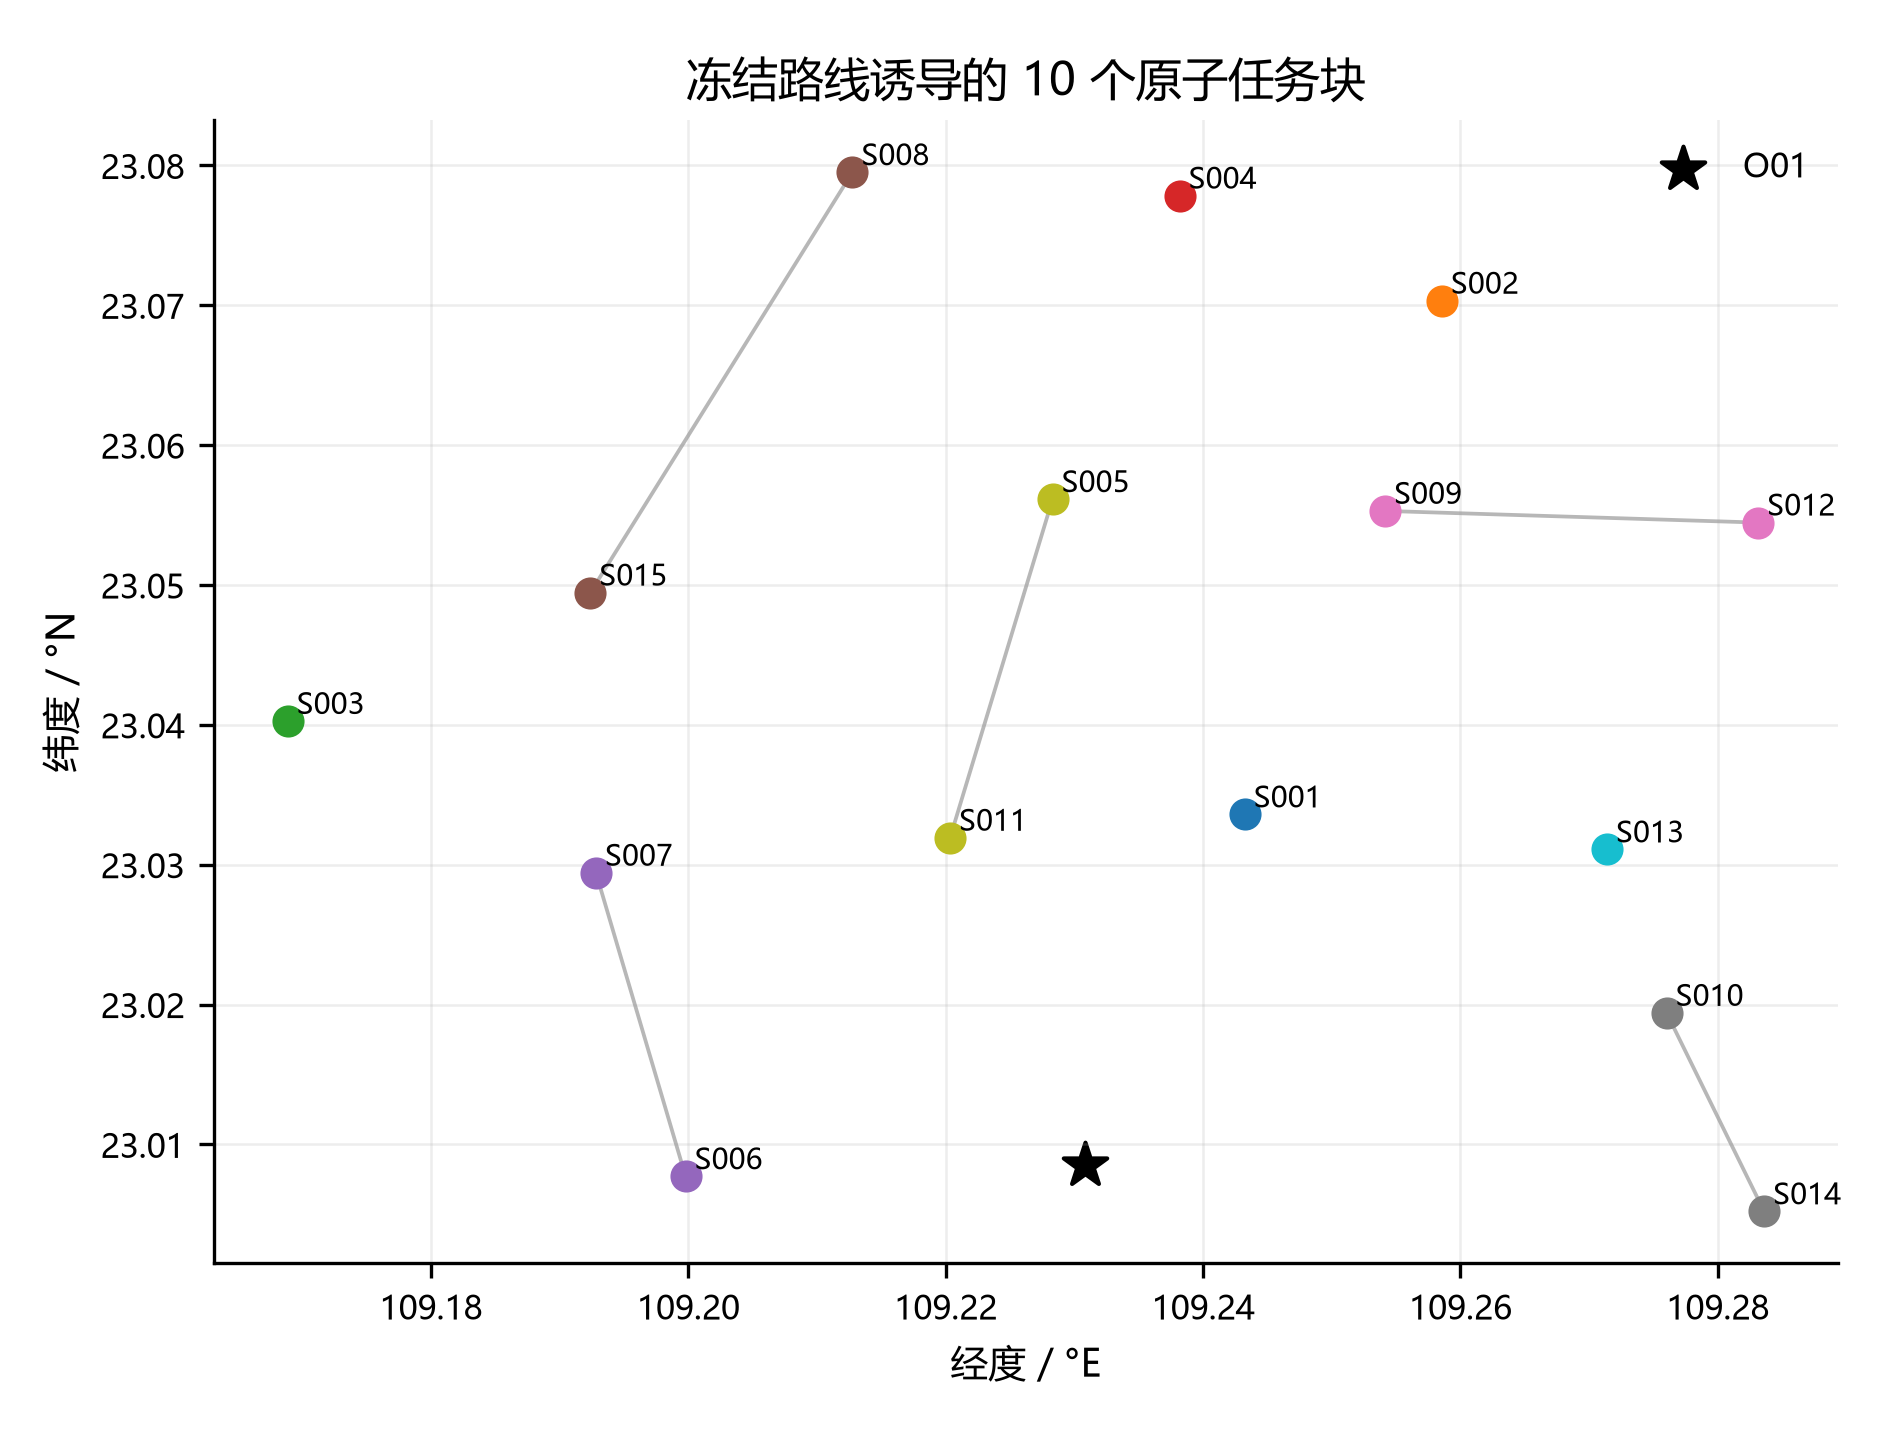
\includegraphics[width=0.78\textwidth]{figures/q3_q4/raw_q4_atomic_components.png}
  \caption{冻结运输路线诱导的11个原子任务块}
  \label{fig:q4-atoms}
\end{figure}

设原子块集合为$\mathcal A=\{A_1,\ldots,A_m\}$，将其划分为$K=2$或3个非空组。令$x_{jk}\in\{0,1\}$表示原子块$j$归属组$k$，则
\begin{equation}
\sum_{k=1}^{K}x_{jk}=1\quad(j=1,\ldots,m),\qquad
\sum_{j=1}^{m}x_{jk}\ge1\quad(k=1,\ldots,K).
\end{equation}
若$m<K$，则该固定运输方案不支持要求的非空分区。原子块由实际路线决定，不能为了获得均衡地图而拆开共访服务区。

\subsection{从实际通信分段确定中继归属}
令$\mathcal R_k$为组$k$承担的运输架次集合，$\mathcal E$为问题三最终通信分段表中出现的“运输架次—中继架次”实际指派关系。该组所需中继任务为
\begin{equation}
\mathcal H_k=\{h:\exists r\in\mathcal R_k,\ (r,h)\in\mathcal E\}.
\label{eq:actual-relay}
\end{equation}
一架中继在某波次内在位，不意味着它实际保障了波次中所有运输任务。必须从通信分段的实际指派提取$\mathcal E$，而不能把整个波次的运输架次清单直接作为保障关系。

若同一中继任务属于多个$\mathcal H_k$，各相关组独立配置资源，并保留其完整悬停点和完整原任务时段。这样既保持题设任务安排不变，又避免把并未服务本组的中继任务错误计入本组。图\ref{fig:q4-flow}给出这一资源归属链。
\begin{figure}[htbp]\centering
\begin{tikzpicture}[node distance=8mm]
\node[block,text width=5.2cm](route)at(0,0){固定运输路线\\建立服务区共访图};
\node[block,text width=5.2cm](comm)at(6,0){最终通信分段\\提取实际运输—中继关系};
\node[block,text width=5.2cm,below=of route](atom){共访连通分量\\形成不可拆原子块};
\node[block,text width=5.2cm,below=of comm](relay){确定各组关联中继\\保留完整任务时段};
\node[block,text width=11.5cm](peak)at(3,-3.4){枚举合法分区；按类型计算无人机、能源资源占用区间峰值};
\node[block,text width=11.5cm,below=of peak](out){比较配置规模、相对集中执行的冗余、库存缺口与工作量均衡};
\draw[edge](route)--(atom);\draw[edge](comm)--(relay);
\draw[edge](atom)--(atom.south|-peak.north);\draw[edge](relay)--(relay.south|-peak.north);
\draw[edge](peak)--(out);
\end{tikzpicture}
\caption{固定方案分区与资源核算流程；不代表已求得的具体服务区分组}\label{fig:q4-flow}
\end{figure}

\subsection{固定时序的最小独立资源数}
对组$k$和资源类型$a$，设必须执行的占用区间集合为$\mathcal I_{ka}$。同型资源可互换、各任务时刻固定且没有额外资源专属约束时，最小配置数等于区间峰值并发数：
\begin{equation}n_{ka}=\max_t\sum_{I\in\mathcal I_{ka}}\ind_I(t).\label{eq:peak}\end{equation}
原因是任何同时占用的区间都必须使用不同实体；反过来，按开始时刻排序、结束后回收资源的贪心分配可用峰值数量完成所有区间。

对运输机按机型分别统计任务区间，对运输电池计入任务后的完整充电；对中继机计入周转，对能源组件计入充电。所有区间采用左闭右开约定，同一时刻结束事件优先于开始事件处理。若未来增加资源专属兼容性、共享充电工位或不同初始SOC，峰值数量不再自动构成充分条件，应扩展资源模型。

\subsection{库存缺口、冗余与组间均衡}
设$I_a$为全局库存，$n_a^{central}$为同一有效联合方案集中执行所需的资源，则
\begin{equation}
D_a^{(K)}=\max\left(0,\sum_kn_{ka}-I_a\right),\qquad
R_a^{(K)}=\sum_kn_{ka}-n_a^{central}.\label{eq:shortage}
\end{equation}
前者描述资源采购或增援缺口，后者描述分区独立执行相对集中执行新增的配置。不能让每个组分别减去一份完整全局库存，也不能把“库存剩余”称为分区冗余。

以组内运输机任务占用时长和中继机含周转的占用时长之和定义工作量$W_k$，不把能源充电时间再次计作无人机机时。均衡性采用总体标准差口径：
\begin{equation}
\bar W=\frac1K\sum_kW_k,\qquad
CV_W=\frac{\sqrt{K^{-1}\sum_k(W_k-\bar W)^2}}{\bar W}.
\end{equation}
另以各组最后返航时刻之差评价完成时间均衡。两者回答不同问题：机时相近的组仍可能因等待或晚开始而较晚结束。

\subsection{分区搜索与比较原则}
按固定顺序逐一分配原子块，并以首次出现的组编号规范化消除标签对称。在每个合法分区上构造$\mathcal R_k$及$\mathcal H_k$，由式\eqref{eq:peak}计算资源向量，再比较缺口、总配置数量、$CV_W$和组间完成时刻极差。跨类型合计仅表示“件数优先”的一种建模偏好，不代表不同资源采购价格相同；同时应完整报告分类型向量，以免合计掩盖资源差异。

对$K=2$固定第一个原子块的标签后，共枚举1023个无重复分区；对$K=3$枚举57002个带标签方案，第2、3组互换后对应28501个无标签分区。全部候选均从通信分段中提取实际“运输架次---中继架次”关系，再计算固定时间轴上的资源峰值。

\subsection{两组与三组的最优分区}
表\ref{tab:q4-groups}给出两种组数下的最优分区及独立资源配置。$K=2$时S001单独组成第1组，其余14个服务区组成第2组；$K=3$时S001和S014分别组成第1、3组，其余13个服务区组成第2组。
\begin{table}[htbp]
  \centering
  \caption{两组与三组最优分区的独立资源配置}
  \label{tab:q4-groups}
  \small
  \begin{tabularx}{\textwidth}{ccYccccl}
    \toprule
    $K$ & 组 & 服务区 & A/B/C型无人机 & A/B/C型电池 & 中继机/组件 & 工作量/h & 完成时刻/s \\
    \midrule
    2 & 1 & S001 & 0/0/1 & 0/0/1 & 0/0 & 0.8858 & 11480.892 \\
    2 & 2 & 除S001外其余14点 & 4/2/1 & 4/3/2 & 2/4 & 20.2107 & 23658.349 \\
    \midrule
    3 & 1 & S001 & 0/0/1 & 0/0/1 & 0/0 & 0.8858 & 11480.892 \\
    3 & 2 & 除S001、S014外其余13点 & 4/1/1 & 4/2/2 & 2/4 & 19.6916 & 23658.349 \\
    3 & 3 & S014 & 0/1/0 & 0/1/0 & 1/1 & 1.4426 & 3024.840 \\
    \bottomrule
  \end{tabularx}
\end{table}

图\ref{fig:q4-tradeoff}按资源类型分别比较库存缺口和相对集中执行的冗余。$K=2$的各类资源总需求均不超过库存，且与集中执行的峰值需求相同；$K=3$需增配1架中继无人机，中继能源组件虽无库存缺口，但相对集中执行多配置1套。关键资源结果见表\ref{tab:q4-resource}。
\begin{figure}[htbp]
  \centering
  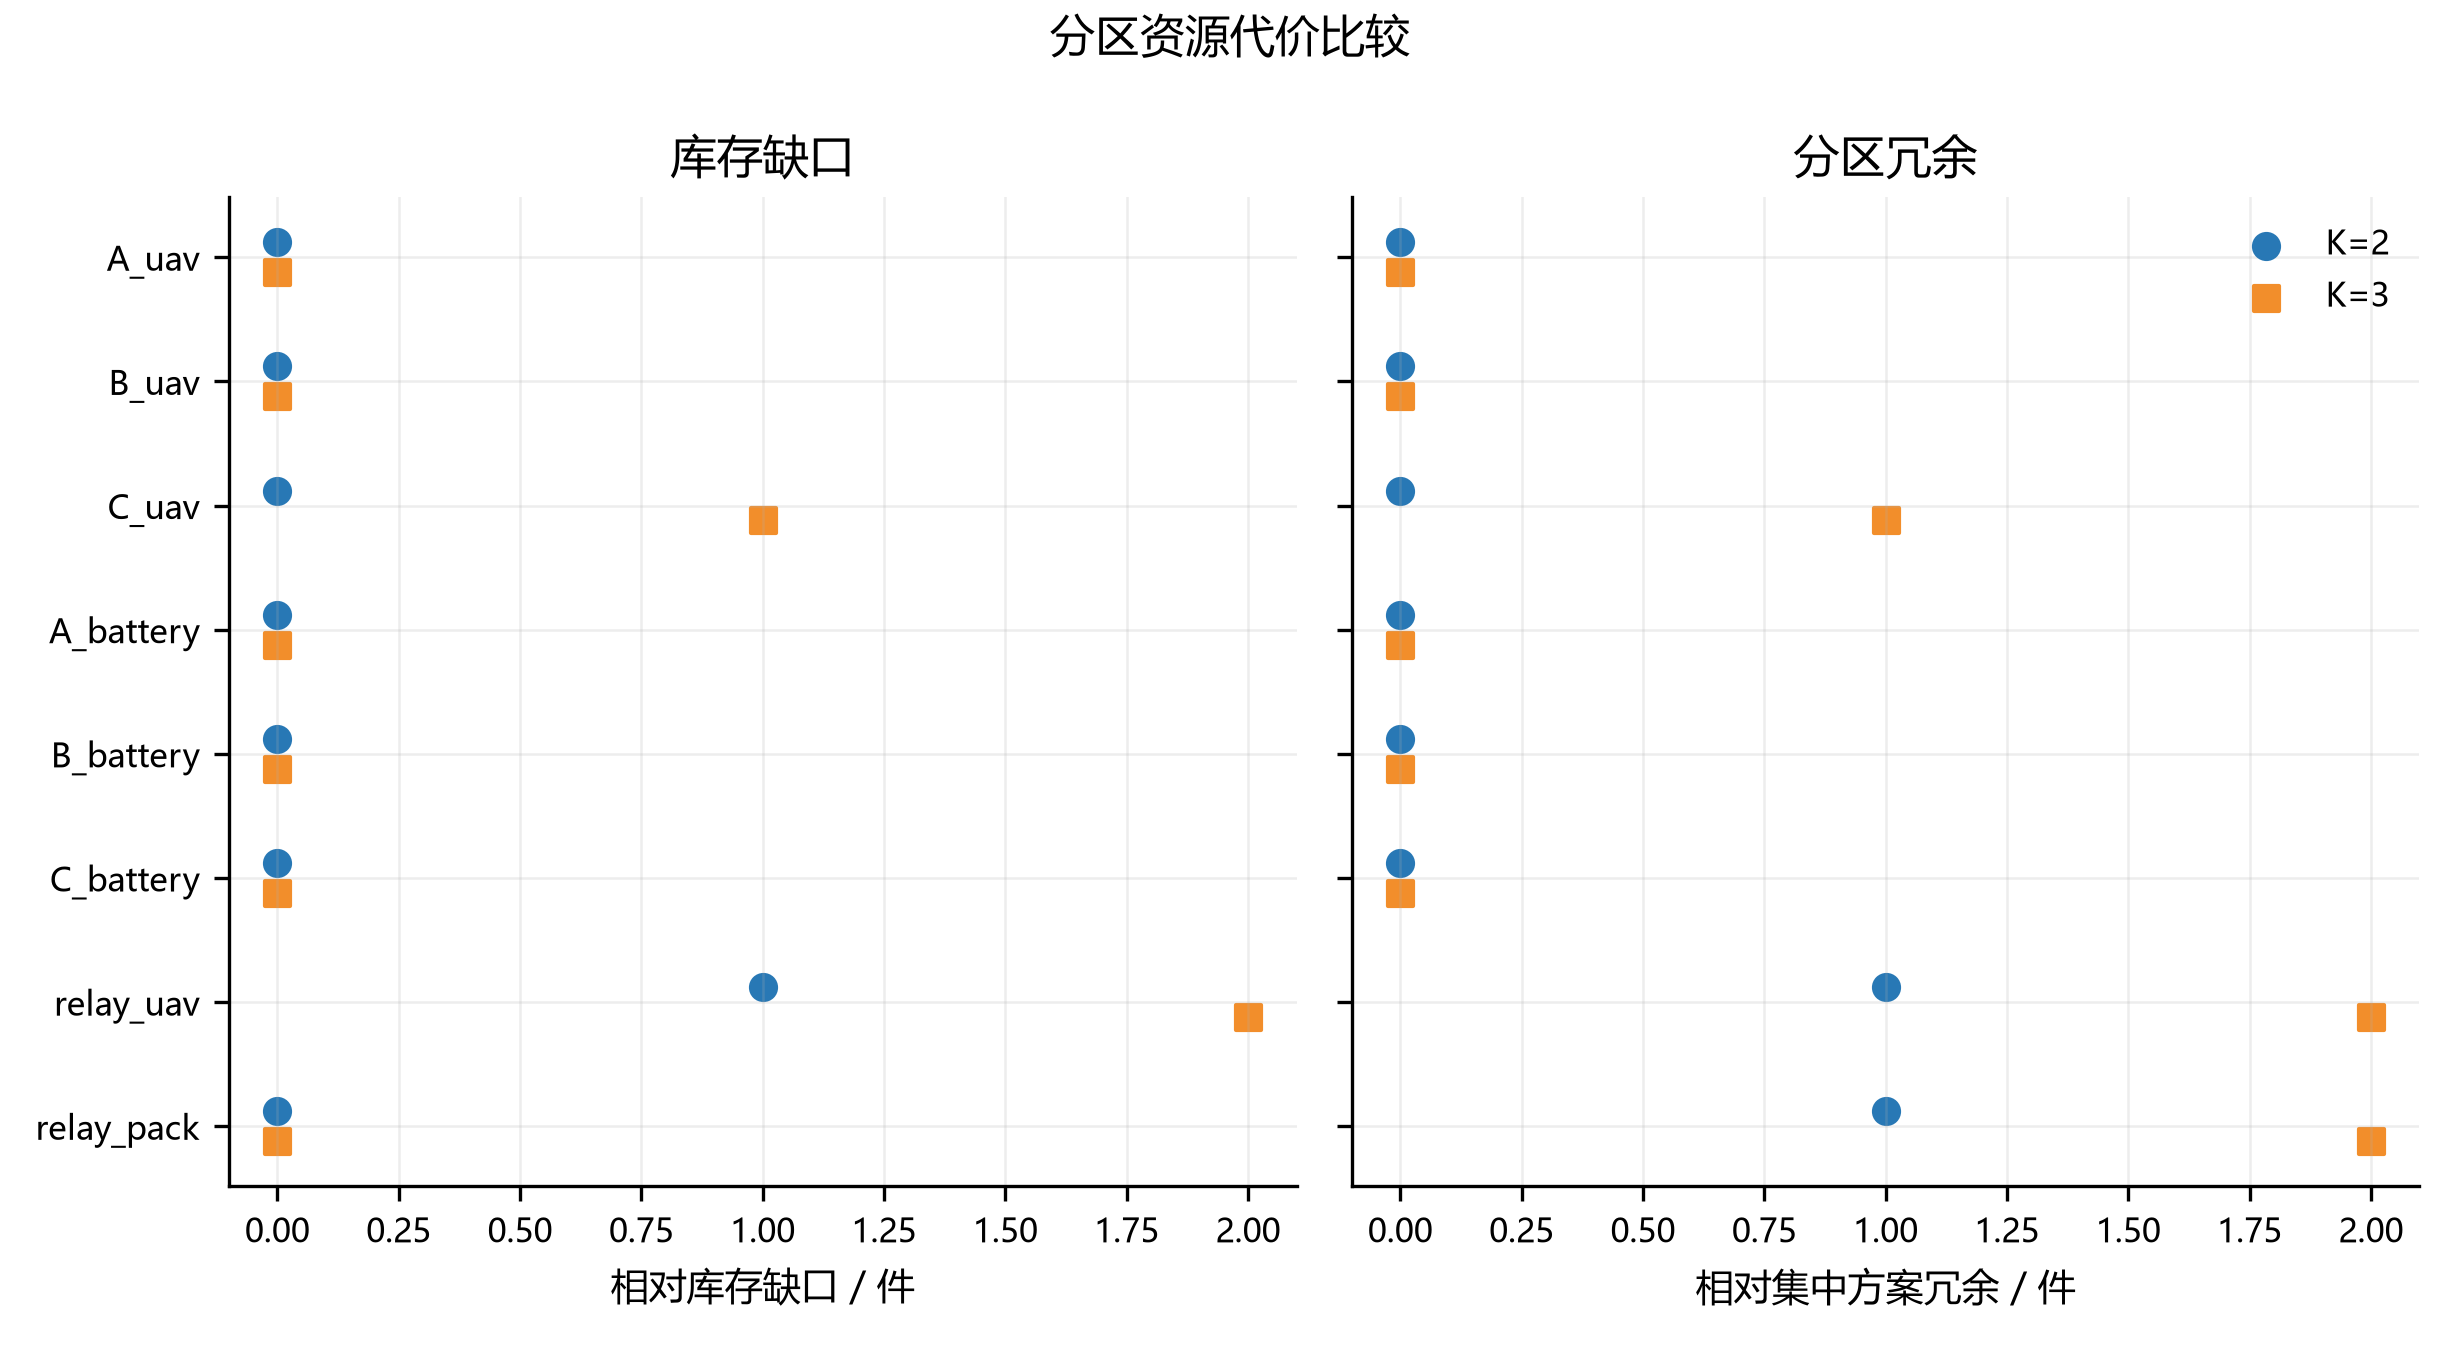
\includegraphics[width=0.98\textwidth]{figures/q3_q4/process_q4_resource_tradeoff.png}
  \caption{两种分区规模的库存缺口与相对集中方案冗余}
  \label{fig:q4-tradeoff}
\end{figure}

\begin{table}[htbp]
  \centering
  \caption{产生缺口或冗余的关键资源}
  \label{tab:q4-resource}
  \begin{tabular}{clrrrrr}
    \toprule
    $K$ & 资源 & 分组总需求 & 库存 & 缺口 & 集中需求 & 分区冗余 \\
    \midrule
    2 & 中继无人机 & 2 & 2 & 0 & 2 & 0 \\
    2 & 中继能源组件 & 4 & 6 & 0 & 4 & 0 \\
    3 & 中继无人机 & 3 & 2 & 1 & 2 & 1 \\
    3 & 中继能源组件 & 5 & 6 & 0 & 4 & 1 \\
    \bottomrule
  \end{tabular}
\end{table}

图\ref{fig:q4-map}给出最优分区的空间位置。空间邻近并不是唯一标准：不可拆性由冻结路线的共访关系决定，资源代价则由运输和通信任务在固定时间轴上的峰值并发决定。
\begin{figure}[htbp]
  \centering
  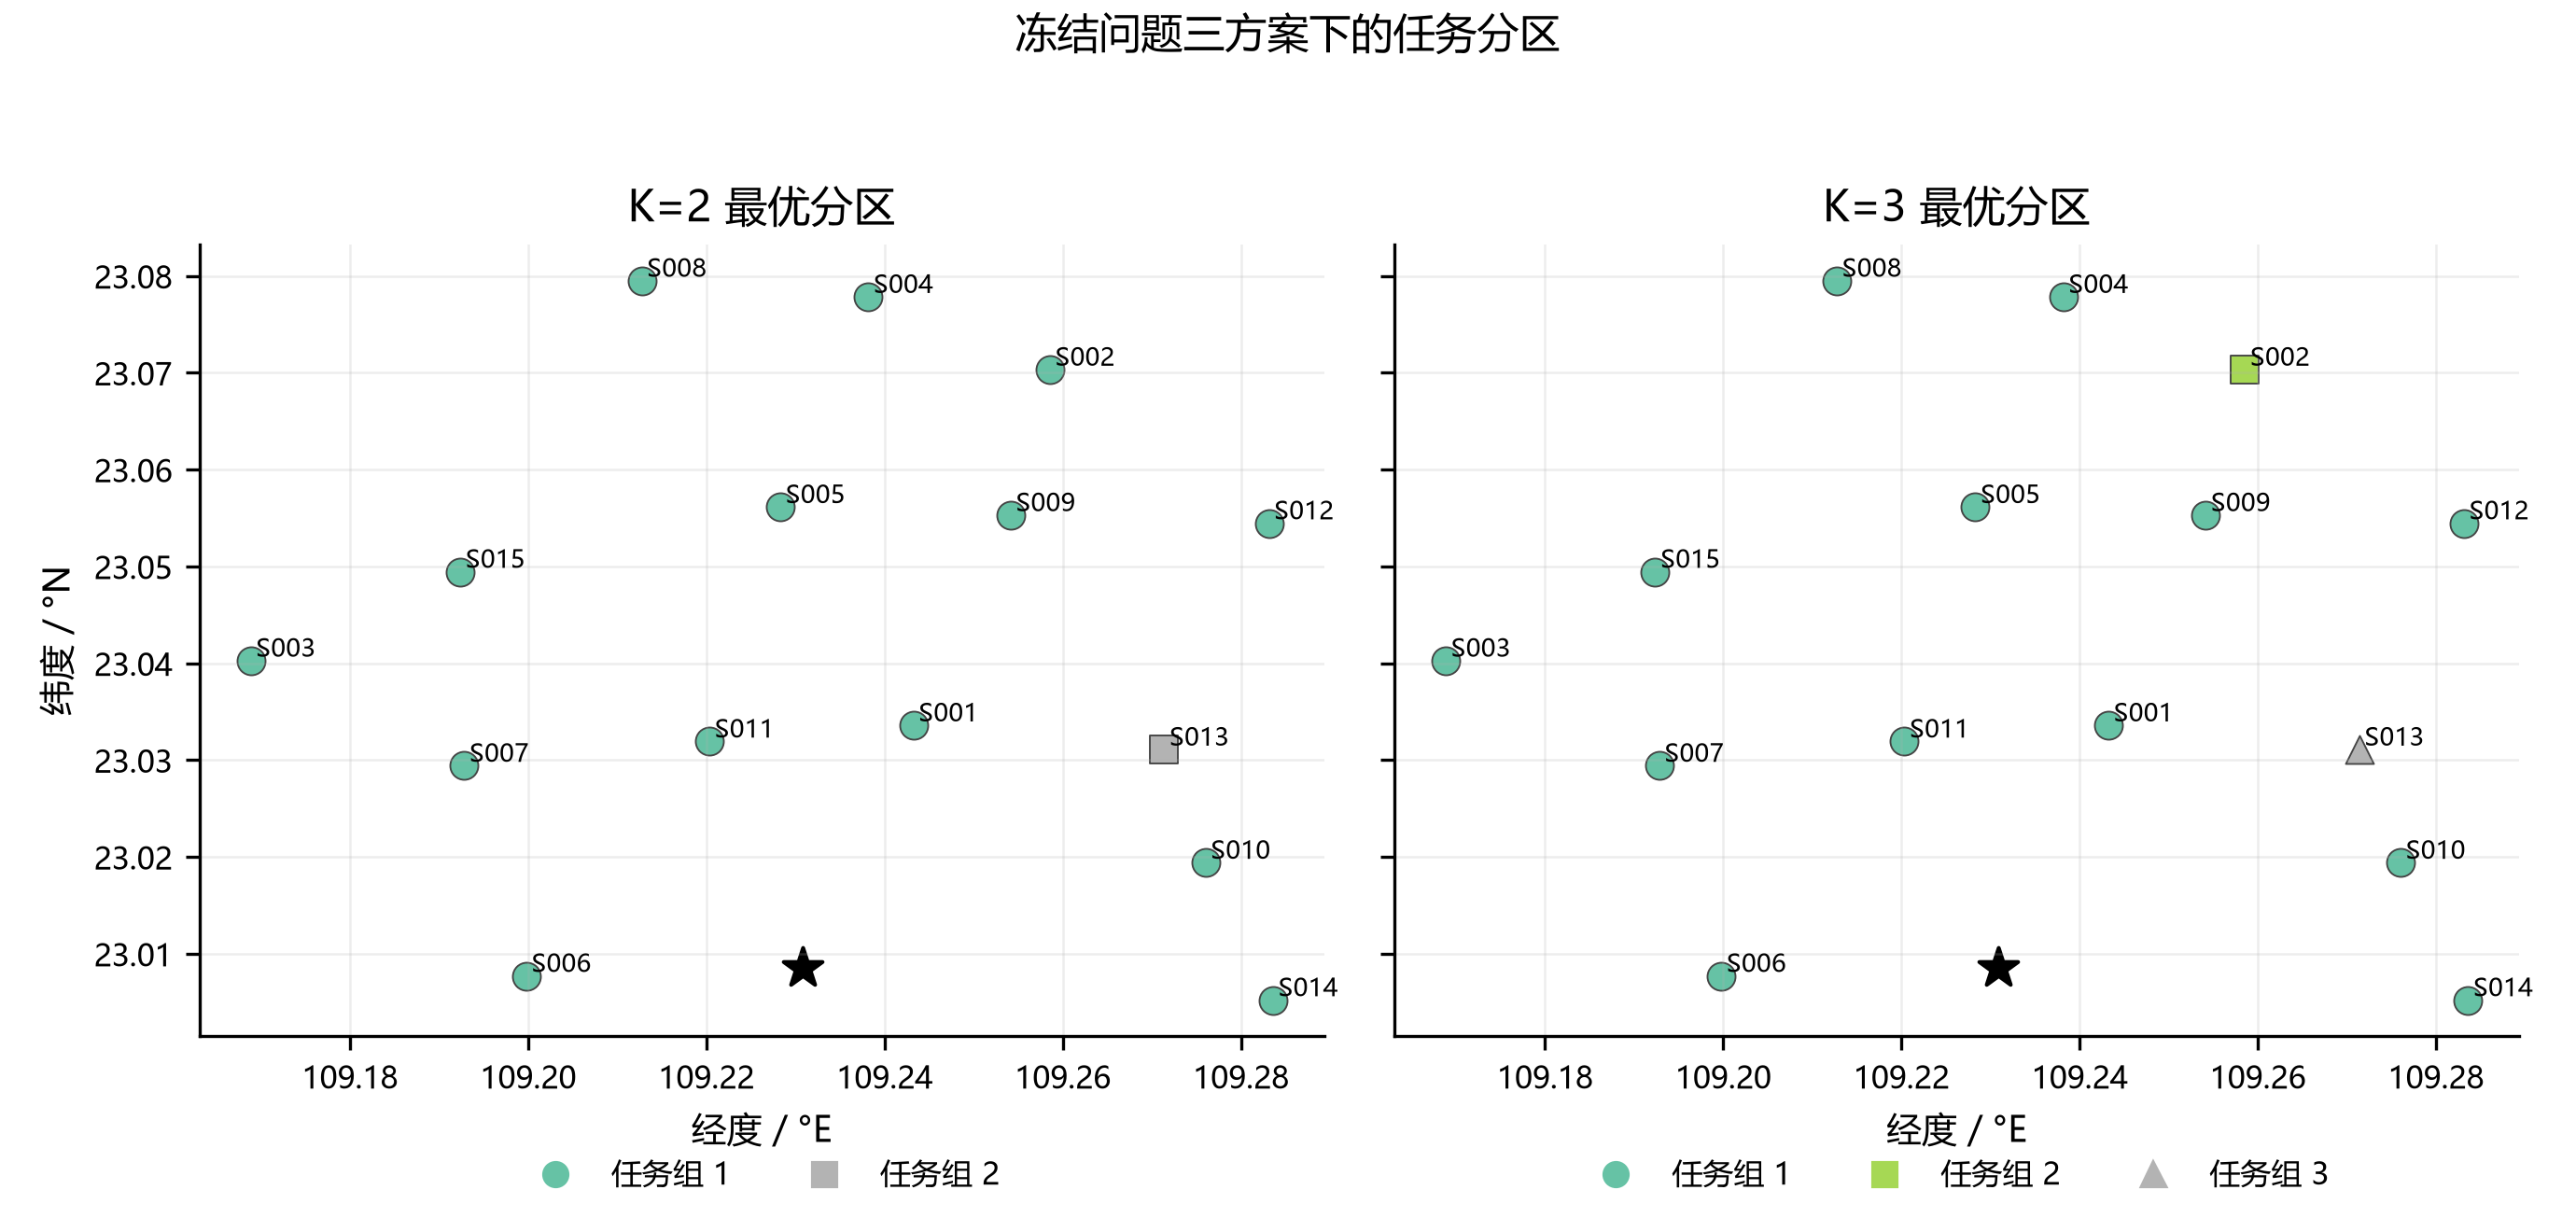
\includegraphics[width=0.98\textwidth]{figures/q3_q4/result_q4_partition_map.png}
  \caption{固定问题三方案下的$K=2$与$K=3$最优任务分区}
  \label{fig:q4-map}
\end{figure}

在“先减少库存缺口，再减少总配置和冗余”的字典序下，$K=2$优于$K=3$：前者无需增配资源，后者缺少1架中继无人机。$K=2$两组工作量分别为0.8858 h和20.2107 h，均衡性较弱，说明资源可实施性与区域负荷均衡存在明显冲突。若管理目标更强调区域自治或负荷均衡，应调整目标优先级，并接受额外的中继资源配置。
